% \documentclass[journal = jpccck, manuscript = article]{achemso}
% \setkeys{acs}{usetitle = true}
% \usepackage{fixltx2e}
% \usepackage{float}
% \usepackage{achemso}
% \usepackage{natbib}
% \usepackage{multirow}
% \usepackage{wrapfig}
% \usepackage{times}
% \usepackage{tablefootnote}
% \usepackage{booktabs}
% \usepackage[version=3]{mhchem}  % this is a great package for formatting chemical reactions
% \usepackage{url}
% \usepackage{graphicx}  % needed for figures
% \usepackage{dcolumn}   % needed for some tables
% \usepackage{bm}        % for math
% \usepackage{amssymb}   % for math
% \usepackage{booktabs}
% \usepackage{tablefootnote}
% \usepackage{mathptmx}

% \newcommand*{\citen}[1]{%
%   \begingroup
%     \romannumeral-`\x % remove space at the beginning of \setcitestyle
%     \setcitestyle{numbers}%
%     \cite{#1}%
%   \endgroup   
% }

\chapter{FRICTION AT ICE-I$_\mathrm{h}$ / WATER INTERFACES IS GOVERNED
  BY SOLID / LIQUID HYDROGEN-BONDING}

% Write a short introduction to the topic discussed in this chapter.

Non-equilibrium molecular dynamics simulations of solid / liquid
friction at ice / water interfaces suggest that the surface density
of solid to liquid hydrogen bonds directly correlates with
interfacial friction.  The basal $\{0001\}$, prismatic
$\{10\bar{1}0\}$, pyramidal $\{20\bar{2}1\}$, and secondary prism
$\{11\bar{2}0\}$ facets of ice-I$_\mathrm{h}$ were drawn through
liquid water with a momentum flux between the solid and liquid
phases. Solid to liquid hydrogen bonds were identified using local
tetrahedral ordering of the water molecules. An expression for
friction coefficients appropriate for negative slip boundary
conditions is presented, and the computed friction of these
interfaces is found to be invariant to the shear rate and direction
of shear relative to the surface features. Structural and dynamic
interfacial widths for all four facets were found to be similar
(6.6--9.5 \AA~structural, 9--15 \AA~dynamic), and are largely
independent of the shear rate and direction. Differences in the
solid to liquid hydrogen bond density are explained in terms of
surface features of the four facets. Lastly, we present a simple
momentum transmission model using the density of solid / liquid
hydrogen bonds, the shear viscosity of the liquid, and the
structural width of the interface.
%\end{abstract}



\begin{table}[h]
\centering
\caption{Computed properties of the
  ice-I$_\mathrm{h}$ interfaces with SPC/E (225~K)
  water. Dynamic widths ($d_\mathrm{10-90}$ and $j_\mathrm{10-90}$)
  are defined in Eqs. \eqref{tauFit} and the discussion section,
  respectively. Uncertainties in the last digit are indicated with
  parentheses.\label{tab:propsSPCE}} 
\begin{tabular}{r|ccc|c}  
  \toprule
  & \multicolumn{3}{c|}{Interfacial Widths (\AA)} & Surface H-bond density \\
  Interface & $w_\mathrm{10-90}$ &  $d_\mathrm{10-90}$ & $j_\mathrm{10-90}$ & $\rho_{sl}$ (\AA\textsuperscript{-2}) \\ 
  \midrule
  Basal  $\{0001\}$                 & 7.5(4) & 11(2) & 11 & 0.1227(3)  \\
  Prismatic  $\{10\bar{1}0\}$       & 7.2(2) & 10(2) & 12 & 0.2014(5)  \\
  Pyramidal  $\{20\bar{2}1\}$       & 6.6(2) & 11(3) & 13 & 0.0866(3)  \\
  Secondary Prism  $\{11\bar{2}0\}$ & 6.7(2) & 11(3) & 10 & 0.1384(4)  \\ 
  \bottomrule
\end{tabular}
\end{table}

\begin{table}[h]
\centering
\caption{Computed properties of the
  ice-I$_\mathrm{h}$ interfaces with TIP4P/Ice (270~K) water. Uncertainties in the last digit are indicated with
  parentheses. \label{tab:propsTIP4P}}
\begin{tabular}{r|ccc|c}  
  \toprule
  & \multicolumn{3}{c|}{Interfacial Widths (\AA)} & 
                                                    Surface H-bond
                                                    density \\
  Interface & $w_\mathrm{10-90}$ &  $d_\mathrm{10-90}$ & $j_\mathrm{10-90}$ & $\rho_{sl}$ (\AA\textsuperscript{-2}) \\ 
  \midrule
  Basal  $\{0001\}$                 & 8.8(8) & 15(3) & 9   & 0.0749(9)\\
  Prismatic  $\{10\bar{1}0\}$       & 9.0(5) & 15(2) & 13  & 0.141(1) \\
  Pyramidal  $\{20\bar{2}1\}$       & 8.2(5) & 13(1) & 10  & 0.074(1) \\
  Secondary Prism  $\{11\bar{2}0\}$ & 9.4(6) & 14(2)   & 12  & 0.119(1) \\
  \bottomrule
\end{tabular}
\end{table}

% These values agree reasonably well with those reported by Haymet
% \textit{et
%   al.}.\cite{Karim1988,Karim1990,Hayward2001,Bryk2002,Hayward2002,Bryk2004}
% Using a variety of water models and several different order
% parameters, they have estimated the ice / water interface to be
% between $5$~\AA~and $18$~\AA~depending on the particular interface and
% means of measure.  For the SPC/E model, they found the basal and
% prismatic ice / water interface to be $\approx 11$~\AA~ wide from
% translational and window-averaged density order parameters. The
% interfacial widths were also estimated by observing the transition of
% a similar tetrahedral order parameter from their ice-like value of
% $0.9$ to the bulk liquid value of $0.6$. This gave estimates of
% $\approx 11$~\AA~, somewhat larger than our current estimates. More
% careful analysis will be necessary to determine if the proton striped
% surface configurations used here are the origin of this discrepancy.




\section{Coefficient of Friction of the Interface}
As liquid water flows over an ice interface, there is a distance from
the structural interface where bulk-like hydrodynamics are recovered.
Bocquet and Barrat constructed a theory for the hydrodynamic boundary
parameters, which include the slipping length
$\left(\delta_\mathrm{wall}\right)$ of this boundary layer and the
``hydrodynamic position'' of the boundary
$\left(z_\mathrm{wall}\right)$.\cite{PhysRevLett.70.2726,PhysRevE.49.3079}
This last parameter is the location (relative to a solid surface)
where the bulk-like behavior is recovered.  Work by Mundy {\it et al.}
has helped to combine these parameters into a liquid-solid friction
coefficient, which quantifies the resistance to pulling the solid
interface through a liquid,\cite{Mundy1997305}
\begin{equation}
\lambda_\mathrm{wall} = \frac{\eta}{\delta_\mathrm{wall}}.
\end{equation}
This expression is nearly identical to one provided by Pit {\it et
  al.} for the solid-liquid friction of an interface,\cite{Pit1999}
\begin{equation}\label{Pit}
  \lambda=\frac{\eta}{\delta}
\end{equation}
where $\delta$ is the slip length for the liquid measured at the
location of the interface itself.  In our simulations, the shoulder on
the velocity profile indicating the location of the hydrodynamic
boundary in the liquid is not always apparent. In some cases, the
linear behavior persists nearly up to the interfacial region.  For
this reason, the hydrodynamic position of the boundary is not always
computable, while the Pit approach (Eq. \ref{Pit}) can be used to find
the solid-liquid friction coefficient more reliably.

In both the Pit and hydrodynamic boundary expressions, $\eta$ is the
shear viscosity of the bulk-like region of the liquid, a quantity
which is easily obtained in VSS-RNEMD simulations by fitting the
velocity profile in the region far from the surface.\cite{Kuang2012}
Assuming linear response in the bulk-like region,
\begin{equation}\label{Kuang}
j_{z}(p_{x})=-\eta \left(\frac{\partial v_{x}}{\partial z}\right)
\end{equation}
Substituting this result into eq. \eqref{Pit}, we can estimate the
solid-liquid coefficient using the slip length,
\begin{equation}
\lambda=-\frac{j_{z}(p_{x})} {\left(\frac{\partial v_{x}}{\partial
      z}\right) \delta}
\end{equation}

For ice / water interfaces, the boundary conditions are no-slip, so
projecting the bulk liquid state velocity profile yields a negative
slip length. This length is the difference between the structural edge
of the ice (determined by the tetrahedrality profile) and the location
where the projected velocity of the bulk liquid intersects the solid
phase velocity (see Figure \ref{fig:delta_example}). The coefficients
of friction for the basal and the prismatic facets were determined for
shearing along both the $x$ and $y$ axes.  The values are given in
table \ref{tab:lambda}. 

Note that the measured friction coefficient for the basal face is
twice that of the prismatic face (regardless of drag direction).
These results may seem surprising as the basalface appears smoother
than the prismatic with only small undulations of the oxygen
positions, while the prismatic surface has deep corrugated channels
along the $x$ direction in the crystal system used in this work.
However, the corrugations are relatively thin, and the liquid phase
water does not appear to populate the channels.  The prismatic face
therefore effectively presents stripes of solid-phase molecules
(making up approximately half of the exposed surface area) with nearly
empty space between them. The interfacial friction appears to be
independent of the drag direction, so flow parallel to these channels
does not explain the lower friction of the prismatic face.  A more
likely explanation is that the effective contact between the liquid
phase and the prismatic face is reduced by the empty corrugations.  

\begin{figure}
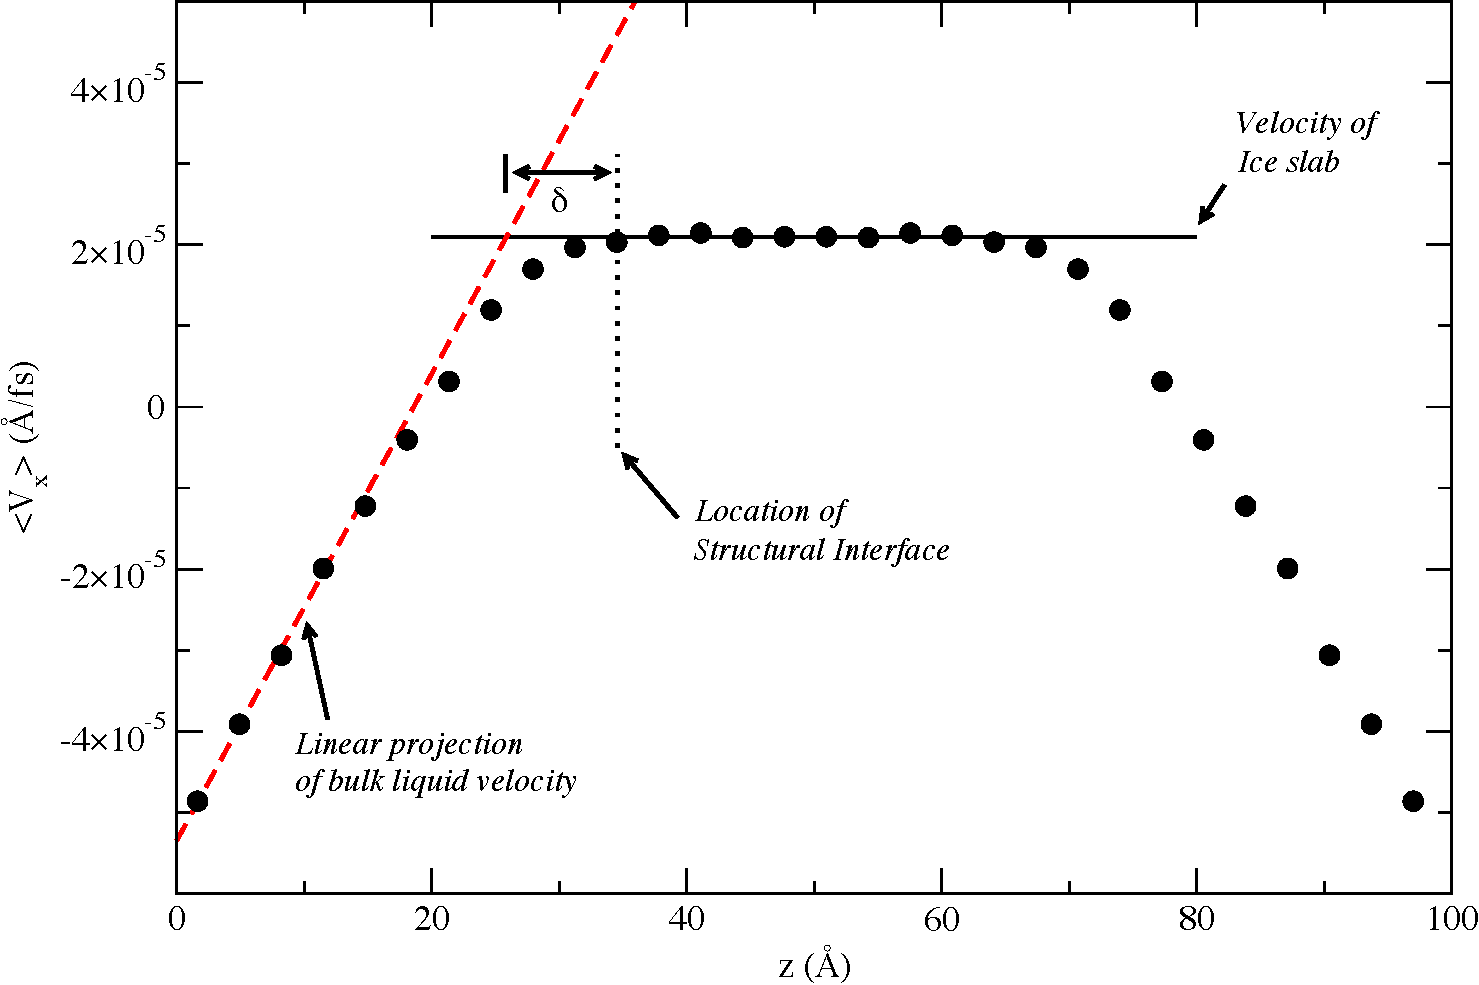
\includegraphics[width=\linewidth]{Figures/delta_example}
\caption{\label{fig:delta_example} Determining the (negative) slip
  length ($\delta$) for the ice-water interfaces (which have decidedly
  non-slip behavior).  This length is the difference between the
  structural edge of the ice (determined by the tetrahedrality
  profile) and the location where the projected velocity of the bulk
  liquid (dashed red line) intersects the solid phase velocity (solid
  black line).  The dotted line indicates the location of the ice as
  determined by the tetrahedrality profile.  This example is taken
  from the basal-face simulation with an applied shear rate of 3.0 ms\textsuperscript{-1}.}
\end{figure}


\begin{table}[h]
\centering
\caption{Solid-liquid friction coefficients (measured in amu~fs\textsuperscript{-1}) }
\label{tab:lambda}
\begin{tabular}{|ccc|}  \hline
           & \multicolumn{2}{c|}{Drag direction} \\ 
 Interface & $x$               & $y$  \\ \hline
     basal &  $0.08 \pm 0.02$  & $0.09 \pm 0.03$ \\
 prismatic & $0.037 \pm 0.008$ & $0.04 \pm 0.01$ \\ \hline
\end{tabular}
\end{table}


\subsection{Solid / liquid friction at ice / water interfaces}
In no-stick boundary conditions, fluid flowing over a solid is
characterized by a slip length, $\delta$, describing the extent of
slip of the fluid at the interface. This length is the extrapolated
distance from the interface where the tangential velocity component
vanishes. For solids with weak interactions with the liquid, there is
little drag imposed on the fluid and the resulting interfacial liquid
velocity, $\Delta v_\mathrm{slip}$, can be significant. In no-stick
boundaries, therefore, the extrapolated slip lengths are also large
(top panel of Fig. \ref{fig:slipLengthPlot}).  Balasubramanian and
Mundy have related the slip length to the interfacial friction
coefficient, 
\begin{equation}\label{kappa1}
\lambda = \frac{\eta}{\delta}
\end{equation}
where $\eta$ is the shear viscosity of the
liquid.\cite{Balasubramanian1999}

For solids that have strong interactions with the liquid, a larger
frictional drag is imposed on the fluid at the interface and the
resulting slip lengths are smaller. When the solid / liquid interactions
become large enough, the interface is best described with stick
boundary conditions, and the slip length will vanish (middle panel of
Fig. \ref{fig:slipLengthPlot}).  Stick boundaries pose a problem for
Eq.  \eqref{kappa1}, as $\lambda$ asymptotically goes to infinity as
$\delta \rightarrow 0$.  Likewise, some materials possess solid / liquid
interactions that are strong enough for the extrapolated tangential
velocity to vanish \textit{before} reaching the solid. The velocity
profile yields a negative slip length (bottom panel of Fig.
\ref{fig:slipLengthPlot}), and the solid / liquid friction coefficient
defined in Eq. \eqref{kappa1} becomes meaningless.  Ice shearing
through liquid water is in the negative slip limit. The tangential
velocity profile of the liquid extrapolates to the solid velocity
several molecular layers before reaching the solid. Thus a new
friction coefficient must be defined to describe these interfaces.

\begin{figure}
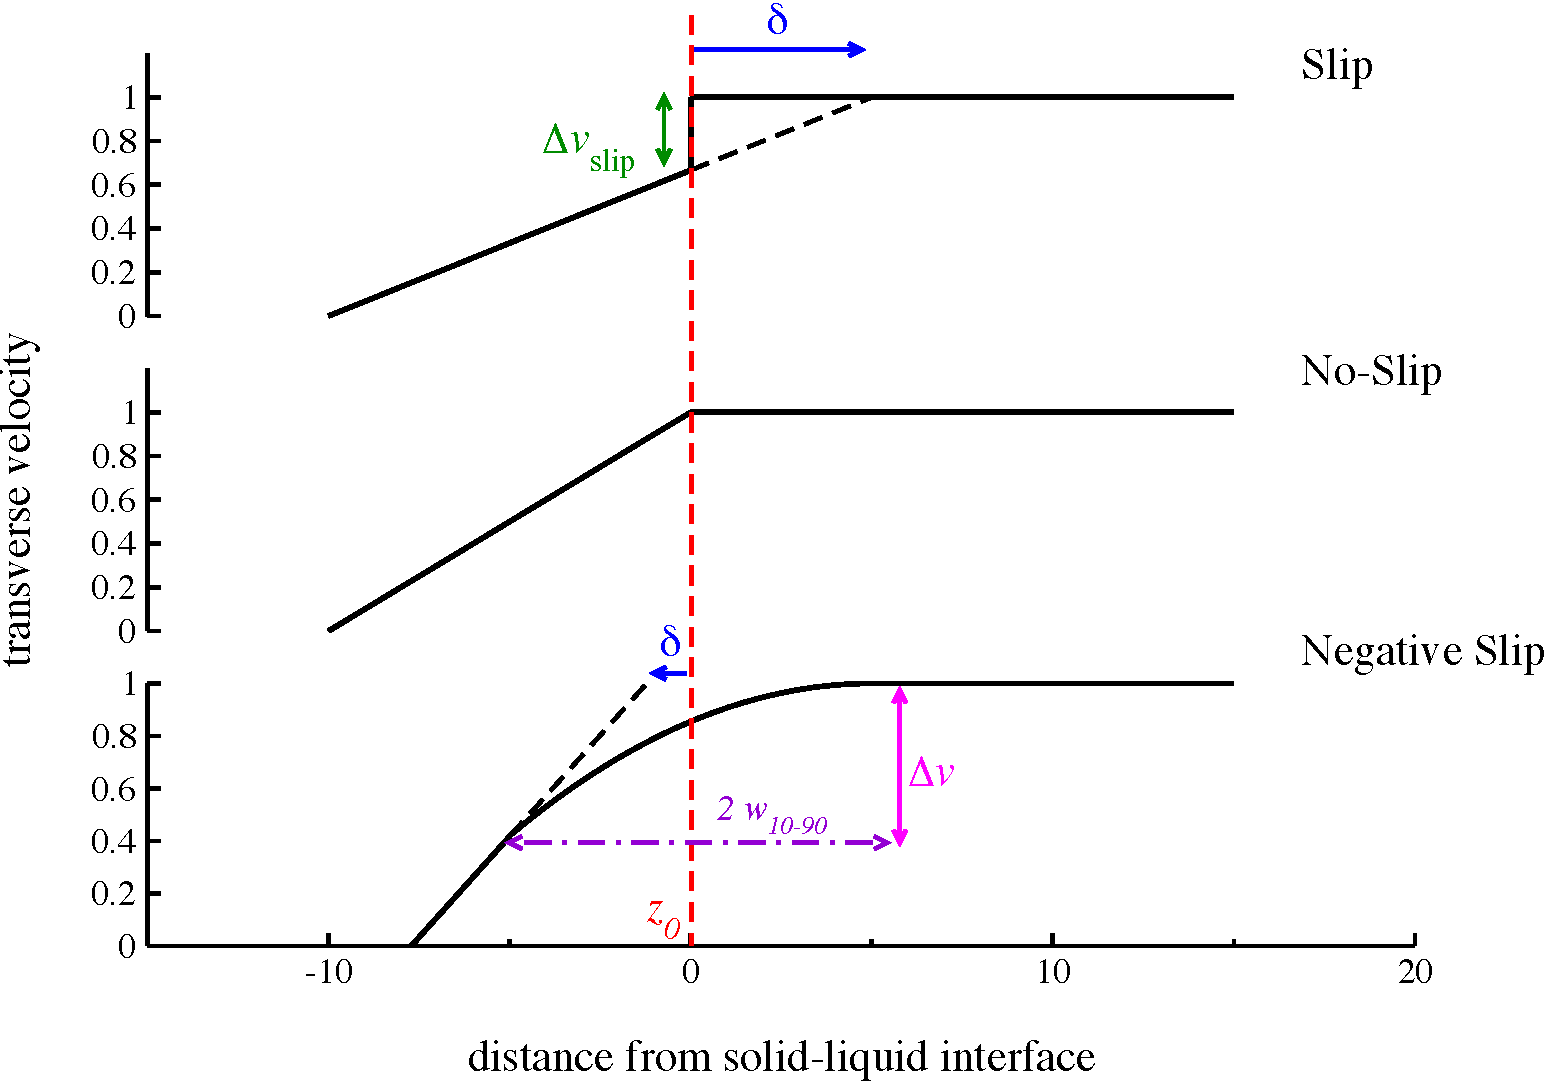
\includegraphics[width=\linewidth]{Figures/slipLengthPlot}
\caption{\label{fig:slipLength} A sketch of transverse velocity
  profiles, $v_x(z)$, for interfaces in slip (top), no-slip (middle),
  and negative slip boundary conditions (bottom).  The location of the
  interface is defined by a Gibbs dividing surface at $z_0$. Under
  negative slip conditions, the 10-90 interfacial width, $w_{10-90}$,
  provides locations that are unambiguously on the liquid and solid
  sides of the interface.\label{fig:slipLengthPlot}}
\end{figure}

A solid / liquid friction coefficient, $\kappa$, may also be defined
using the velocity drop across the interface, rather than the length
scale over which this drop occurs. We can relate the imposed shear
stress with the relative tangential velocity of the fluid in the
interfacial region,\cite{Kuang2012}
\begin{equation}\label{Shenyu-13}
j_{z}(p_{x}) = \kappa_{x} \Delta v
\end{equation}
where $\Delta v = v_{x}(\mathrm{solid}) - v_{x}(\mathrm{liquid})$ is
the difference in transverse velocity between points that are
unambiguously on the solid and liquid sides of the interface.  In slip
boundary conditions, $\kappa$ and $\lambda$ are identical, but
Eq. \eqref{Shenyu-13} provides a direct analogy to non-equilibrium
expressions for the interfacial thermal conductance $(G)$,
\begin{equation}
J_z = G~ \Delta T.
\end{equation}
Here, $J_z$ is a thermal flux and the temperature drop is measured
across an interface of \textit{finite width}. By analogy, $\kappa$ is
a transport coefficient that measures \textit{interfacial momentum
  conductance} across an interface of finite width.

In ice / water interfaces, the solid / liquid boundary is not
an infinitely thin plane. An order parameter (the tetrahedrality) goes
smoothly between the phases over a few molecular diameters.  We can
use this order parameter to find the interfacial width and define
locations in space that are unambiguously on the solid and liquid
sides of the interface.  In what follows, we have used the Gibbs
dividing surface ($z_0$) and the 10$-$90 width of the interface
($w_\mathrm{10-90}$) to arrive at physical locations for measuring
$v_{x}(solid)$ and $v_{x}(liquid)$.  These uniquely define a friction
coefficient in terms of well-defined structural features ($z_0$ and
$w_\mathrm{10-90}$) and dynamic properties ($v_{x}(z)$) of the
interface.

Tangential velocity profiles from the simulations were fit using a
piecewise function that is both continuous and continuously
differentiable. The velocity profiles, $v_x(z)$, obtained from each
shearing simulation were fit assuming linear behavior through each of
the three regions of the simulation box; the lower liquid, the solid,
and the upper liquid. Parabolic functions were designed to capture the
negative slip behavior that links the three regions,
\begin{equation}\label{vfit}
v(z) =
\begin{cases}
  v_{l} - m_{l}z & 0 \leq z < (z_{1} - w) \\
  v_{s} - \frac{1}{2}k(z-z_{1})^{2} & (z_{1}-w) \leq z < z_{1} \\
  v_{s}  & z_{1} \leq z < z_{2} \\
  v_{s} - \frac{1}{2}k(z-z_{2})^{2}  & z_{2} \leq z <( z_{2} + w)\\
  v_{s} - \frac{1}{2}kw^{2} - m_{l}(z-(z_{2} + w)) & (z_{2} + w) \leq z \\
\end{cases}
\end{equation}
  
Here, $v_{l}$ is the velocity of the liquid at the middle of the
liquid domain (the edge of the simulation box), and $v_{s}$ is the
velocity of the solid. The locations $z_{1}$ and $z_{2}$ are the edges
of the ice slab, and $w$ is the width of the interface (distinct from
$w_{10-90}$ mentioned in the main text). The parameter $m_{l}$ is the
slope of the velocity profile in the liquid regions of the box which
is related to the liquid-state viscosity. Figure \ref{fig:pyrComic}
shows a representative velocity profile (navy squares) and fit (green
line) with the locations of $z_{1}$ and $z_{2}$ indicated as vertical
dotted lines. Once the fits were obtained, the values for
$v_{x}(solid)$ and $v_{x}(liquid)$ for Eq. (5) were sampled from the
fit. The $z$ locations used to sample the fit were determined by
structural measures. The $z$ location for $v_{x}(liquid)$ was taken to
be the Gibbs dividing surface of the interface, less the 10$-$90 width
of the interface. Similarly, the $z$ location for $v_{x}(solid)$ was
taken to be the Gibbs dividing surface plus the 10$-$90 width of the
interface.

To arrive at estimates of
the interfacial velocities, these fits were queried at locations on
either side of the structural Gibbs dividing surface,
\begin{align}
v_{x}(\mathrm{solid}) & = v_{x}( z_0 + w_\mathrm{10-90})  \label{eq:vx1}\\
v_{x}(\mathrm{liquid}) & = v_{x}( z_0 - w_\mathrm{10-90}). \label{eq:vx2}
\end{align}
The momentum flux, $j_{z}(p_{x})$ is an imposed parameter of the
VSS-RNEMD simulations, and by using Eq. \eqref{Shenyu-13}, estimates
of interfacial friction coefficient $\kappa$ are straightforward.

The calculated $\kappa$ values found for the four crystalline facets
of ice-I$_\mathrm{h}$ investigated here are shown in Table
\ref{tab:kappa}. Solid / liquid friction coefficients for shearing
simulations where the imposed momentum flux was in the $y$-dimension,
$\kappa_{y}$, are calculated in the same manner, with $j_{z}(p_{y})$
and $v_{y}$ substituting for $j_{z}(p_{x})$ and $v_{x}$ in
Eqs. \eqref{Shenyu-13}, \eqref{eq:vx1}, and \eqref{eq:vx2}.  These
results were found to be independent of the shear rate (see
Fig. \ref{fig:kappaPlot}), as well as the direction of the shear
relative to the features on the surfaces of the facets.


\begin{figure}
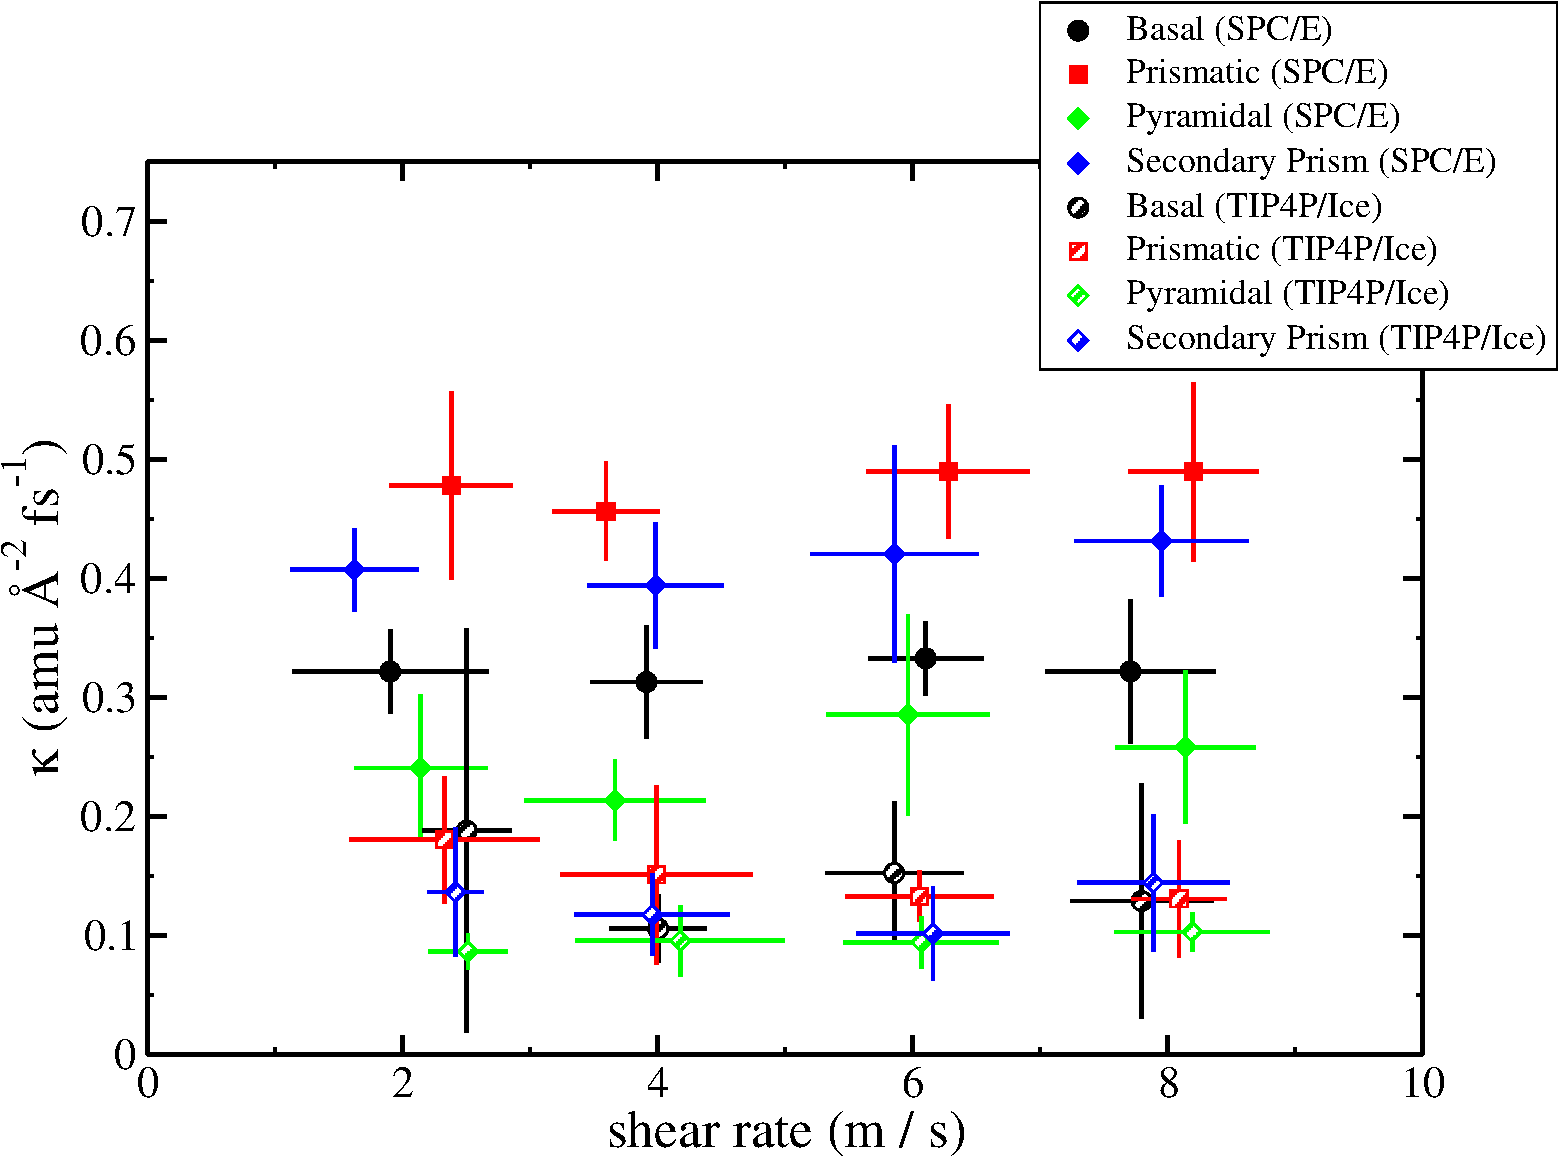
\includegraphics[width=\linewidth]{Figures/kappaPlot2}
\caption{\label{fig:kappaPlot} Dependence on the observed friction
  coefficient on the shear rate of the ice through the surrounding
  liquid water.  The RNEMD simulations impose a momentum flux, but the
  resulting shear rates can vary.  Here, we collect data in 2 m/s bins
  to accumulate statistics over multiple independent simulations.  The
  SPC/E simulations (solid symbols) were done at 225K, and the
  TIP4P/Ice simulations (patterned symbols) were carried out at
  270K. The points on this plot have also been averaged over shear
  direction ($x$ and $y$).}
\end{figure}


\begin{table}[h]
\centering
\caption{Solid / liquid friction coefficients (in units of amu \AA\textsuperscript{-2} fs\textsuperscript{-1}) for
  ice-I$_\mathrm{h}$ interfaces with water. Uncertainties in the last digit are indicated with
  parentheses.\label{tab:kappa}}
\begin{tabular}{r|cc|cc}  
  \toprule
  & \multicolumn{2}{c|}{SPC/E (225~K)} & \multicolumn{2}{c}{TIP4P/Ice (270~K)} \\
  Interface & $\kappa_{x}$ &  $\kappa_{y}$ & $\kappa_{x}$ &  $\kappa_{y}$ \\ 
  \midrule
  Basal  $\{0001\}$                 & 0.32(5)  & 0.31(4) & 0.12(2)  & 0.13(2) \\
  Prismatic  $\{10\bar{1}0\}$       & 0.44(5)  & 0.46(5) & 0.16(2)  & 0.16(3) \\
  Pyramidal  $\{20\bar{2}1\}$       & 0.28(3)  & 0.25(3) & 0.09(1)  & 0.10(1) \\
  Secondary Prism  $\{11\bar{2}0\}$ & 0.44(4)  & 0.42(5) & 0.14(3)  & 0.14(2) \\ 
  \bottomrule
\end{tabular}
\end{table}

Note that the values of $\kappa$ for the basal and prismatic crystal
facets in Table \ref{tab:kappa} disagree with values for interfacial
friction ($\lambda$) we previously reported.\cite{Louden2013a} In our
initial report, the expression for the coefficient of friction was
derived from equation \eqref{kappa1} and the linear constitutive
relation for shear stress in a bulk fluid.  However, as described
above, sheared ice / water interfaces are in the domain negative slip
lengths. Eq. \eqref{kappa1} should only be used in slip boundary
conditions, as negative slip can yield coefficients of friction that
appear to be smaller in magnitude than the zero slip conditions. In
our previous work, the prismatic surface was found to have a larger
negative slip length than the basal face, indicating a prismatic
surface that should have been reported with a larger coefficient of
friction. If one instead uses Eq. \eqref{Shenyu-13} and interfacial
widths to compute friction, the reported values come into agreement.

The two water models give two significantly different values for the
friction coefficients. This is primarily a result of the difference in
water viscosities at the two coexistence temperatures ($\eta = $ 15.9
cP for SPC/E at 225K and 6.1 cP for TIP4P/Ice at 270K), which alters
the stream velocity on the liquid side of the interface. The relative
ratios of facet friction are similar in both models, however, with
$\kappa_\mathrm{prismatic} / \kappa_\mathrm{basal} =$ 1.56~(SPC/E) and
1.32~(TIP4P/Ice),
$\kappa_\mathrm{pyramidal} / \kappa_\mathrm{basal} =$ 0.84~(SPC/E) and
0.81~(TIP4P/Ice), and
$\kappa_\mathrm{secondary} / \kappa_\mathrm{basal} =$ 1.33~(SPC/E) and
1.15~(TIP4P/Ice). The observed ordering of facet friction
coefficients,
\begin{equation}
\kappa_\mathrm{pyramidal} < \kappa_\mathrm{basal} <
\kappa_\mathrm{secondary} < \kappa_\mathrm{prismatic} 
\end{equation} 
seems robust.

 
\section{Discussion}
The primary result of this paper is the observation that the different
facets of ice-I$_\mathrm{h}$ produce significantly different solid /
liquid interfacial friction coefficients with water (see Table
\ref{tab:kappa}).  The two prismatic surfaces displayed the largest
coefficients of friction, while the basal and pyramidal facets
exhibited significantly lower friction. This trend is robust over a
wide range of shear rates, and shear direction relative to ice surface
features. Also, while the magnitude of the solid / liquid friction
coefficients differ due to liquid viscosities, the facet trends are
exhibited by both SPC/E and TIP4P/Ice at their coexistence
temperatures.

It is surprising that the observed solid / liquid friction
coefficients do not depend on the shear direction relative to surface
features. Pfalzgraff \textit{et al.} have recently investigated
diffusion of the water molecules comprising the QLL on the vacuum
exposed basal, prismatic, and pyramidal surfaces of an
ice-I$_\mathrm{h}$ crystal.\cite{Pfalzgraff2011} They observed
anisotropic diffusion on the prismatic and pyramidal surfaces at 250~K
with the NE6 model ($\sim$~40~K below the melting temperature of that
model). In two following studies, Gladich \textit{et al.}
investigated the temperature dependence of this phenomena and deduced
the mechanism of anisotropic self-diffusivity at the prismatic
ice-vapor interface.\cite{Gladich2011,Gladich2015} They observed a
transition from anisotropic to isotropic diffusion at about 260~K with
the NE6 model, and attributed the transition to a change in the
prevailing mechanism of self-diffusion. At temperatures colder than
260~K, the QLL is sparse and the diffusing molecules are strongly
influenced by the underlying geometry of the crystal. At temperatures
warmer than 260~K, the QLL is thicker and diffusion occurs at the
outer part of the QLL. These results were robust for TIP4P/2005 and
TIP5P-Ew at the same relative undercooling temperature. Since our ice
/ water interfaces are at their respective coexistence temperatures,
the effects of the underlying ice crystal may be masked and we might
expect to recover isotropic behavior.

The differences in friction are also surprising given that densities
and molecular interactions are identical for the four interfaces and
the interfacial widths measured via both structural and dynamic
features are also quite similar (for the interfaces treated with the
same water model). There are few remaining surface properties that
could give rise to differences in solid / liquid friction of the four
facets, notably surface corrugation, hydrogen bonding density, and
hydrogen bond lifetime at the interface. In this section we
investigate the roles of these surface features.

\subsubsection{Solid / liquid hydrogen bond density}
The four ice surfaces may potentially have different densities of
hydrogen bonds that bridge the solid and liquid. An ice surface that
forms more hydrogen bonds with the interfacial liquid would be able to
exert significant lateral forces on the liquid layer, yielding a
larger friction coefficient. To probe this possibility, we have
investigated the density of cross hydrogen bonds between the ice and
the liquid.

Quantifying water molecules as ``ice'' or ``liquid'' at an interface
of finite width requires a local order parameter for separating the
molecules.  Conde \textit{et al.}\cite{Conde2008} (and later Gladich
\textit{et al.}\cite{Gladich2011,Gladich2015}) discriminated molecules
as either ``ice'' or ``liquid'' by a threshold value of the local
tetrahedral order parameter (the same order parameter described here
in section \ref{structure}), denoted $q_{t}$. This threshold value was
obtained by equating the probability of incorrectly assigning a
liquid-like molecule as ice-like to the probability of incorrectly
assigning an ice-like molecule as liquid-like. Molecules with
$q < q_{t}$ were denoted as liquid-like, while those found having
$q > q_{t}$ were designated ice-like.

In a similar manner, we have chosen a threshold value of the local
tetrahedral order parameter as our partitioning criterion. Here,
$q_{t}$ is taken to be the value of the order parameter at the Gibbs
dividing surface ($q(z_0) \approx 0.84$ for SPC/E and
$q(z_0) \approx 0.85$ for TIP4P/Ice).  Note that some molecules have
strong tetrahedral ordering in the liquid phase, so this segregation
will not yield perfect division between ice and liquid phase
molecules.

To determine if a hydrogen bond has been formed between two water
molecules, we used the geometric criteria of Luzar and
Chandler.\cite{Luzar1996} We identify a hydrogen bond between two
water molecules if the distance between their oxygen sites,
$r_\mathrm{OO} < 3.5$~\AA, and the OHO bond angle,
$\theta_\mathrm{OHO} < 30^\circ$.

For each of the shearing simulations performed above, a hydrogen bond
tetrahedrality matrix was constructed.  Snapshots from the shearing
trajectories were taken every $0.1$ ps, and the tetrahedrality $(q)$
value for each water molecule in the system was calculated. Hydrogen
bonds were also identified, and the tetrahedrality of the donor
$(q_{D})$ and acceptor $(q_{A})$ molecules were recorded. A
probability density of hydrogen bonds categorized by donor and
acceptor tetrahedrality, $\rho_\mathrm{HB}(q_D, q_A)$, was then
recorded.

\begin{figure}
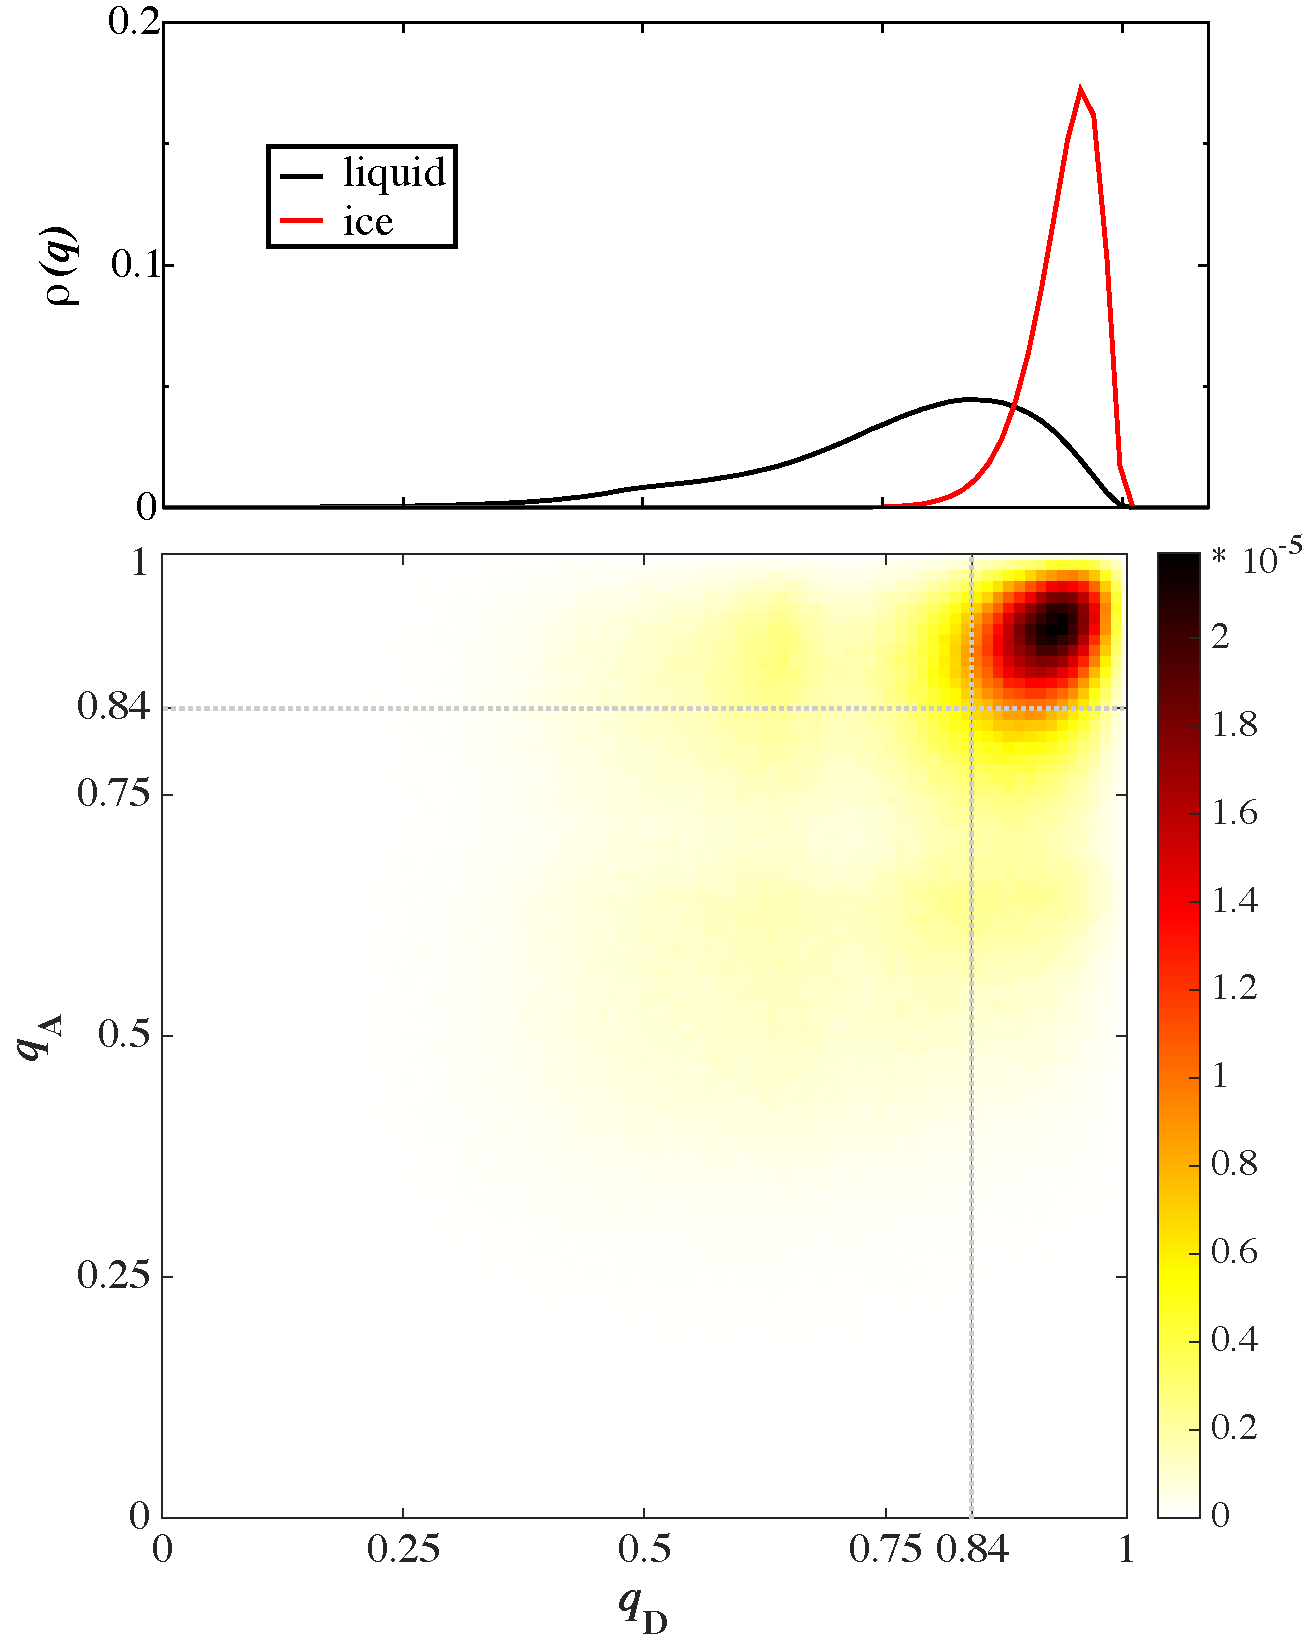
\includegraphics[width=5in]{Figures/hbtet.pdf}
\caption{\label{fig:tetHBMatrix} Distribution of hydrogen bonds at a
  prismatic interface showing the tetrahedralities of donor $(q_D)$
  and acceptor $(q_A)$ molecules (lower panel). Distributions of
  tetrahedralities in bulk ice and liquid phases are shown in the
  upper panel. The value of $q$ at the Gibbs dividing surface is
  indicated with dashed lines. Hydrogen bonds between ice molecules
  are represented by the upper right square, while those between
  liquid molecules are in the lower left.  Hydrogen bonds that bridge
  the ice-liquid interface exist primarily in the vertical and
  horizontal strips that remain.}
\end{figure}

The lower panel of Fig. \ref{fig:tetHBMatrix} shows a hydrogen bond
tetrahedrality distribution for the prismatic facet with $q_{D}$
plotted along the $x$-axis and $q_{A}$ along the $y$-axis.  Population
around $q_{D} \approx q_{A} \approx 0.9$ indicates the density of
ice-ice hydrogen bonds in the system, while the liquid-state hydrogen
bonds are concentrated in the lower left, and are significantly more
diffuse.  The off-diagonal regions of the distribution represent the
population of molecules in tetrahedral (ice-like) environments bound
to non-tetrahedral (liquid-like) environments. Integrating the
population found in each of these regions and normalizing by the
surface area of each ice crystal produces a surface density of
hydrogen bonds (\AA\textsuperscript{-2}) formed between the ice and
interfacial liquid,
\begin{equation}\label{hbondDensity}
\rho_{sl} = \frac{N_\mathrm{HB}}{2 L_{x}L_{y}} \left[ \int_0^{q_{t}}
  dq_{D} \int_{q_{t}}^1 dq_{A}~\rho_\mathrm{HB}(q_{D},q_{A}) +  \int_0^{q_{t}}
  dq_{A} \int_{q_{t}}^1 dq_{D}~\rho_\mathrm{HB}(q_{D},q_{A}) \right]
\end{equation}
$N_\mathrm{HB}$ is the total number of hydrogen bonds found in the
system, and $L_x$ and $L_y$ are the dimensions of the two ice facets
exposed to the liquid.  Values for $\rho_{sl}$ for each of the ice
surfaces are reported in Table \ref{tab:propsSPCE} and \ref{tab:propsTIP4P}.

\begin{table}[h]
\centering
\caption{Computed properties of the
  ice-I$_\mathrm{h}$ interfaces with SPC/E (225~K)
  water. Dynamic widths ($d_\mathrm{10-90}$ and $j_\mathrm{10-90}$)
  are defined in Eqs. \eqref{tauFit} and the discussion section,
  respectively. Uncertainties in the last digit are indicated with
  parentheses.\label{tab:propsSPCE}} 
\begin{tabular}{r|ccc|c}  
  \toprule
  & \multicolumn{3}{c|}{Interfacial Widths (\AA)} & Surface H-bond density \\
  Interface & $w_\mathrm{10-90}$ &  $d_\mathrm{10-90}$ & $j_\mathrm{10-90}$ & $\rho_{sl}$ (\AA\textsuperscript{-2}) \\ 
  \midrule
  Basal  $\{0001\}$                 & 7.5(4) & 11(2) & 11 & 0.1227(3)  \\
  Prismatic  $\{10\bar{1}0\}$       & 7.2(2) & 10(2) & 12 & 0.2014(5)  \\
  Pyramidal  $\{20\bar{2}1\}$       & 6.6(2) & 11(3) & 13 & 0.0866(3)  \\
  Secondary Prism  $\{11\bar{2}0\}$ & 6.7(2) & 11(3) & 10 & 0.1384(4)  \\ 
  \bottomrule
\end{tabular}
\end{table}

\begin{table}[h]
\centering
\caption{Computed properties of the
  ice-I$_\mathrm{h}$ interfaces with TIP4P/Ice (270~K) water. Uncertainties in the last digit are indicated with
  parentheses. \label{tab:propsTIP4P}}
\begin{tabular}{r|ccc|c}  
  \toprule
  & \multicolumn{3}{c|}{Interfacial Widths (\AA)} & 
                                                    Surface H-bond
                                                    density \\
  Interface & $w_\mathrm{10-90}$ &  $d_\mathrm{10-90}$ & $j_\mathrm{10-90}$ & $\rho_{sl}$ (\AA\textsuperscript{-2}) \\ 
  \midrule
  Basal  $\{0001\}$                 & 8.8(8) & 15(3) & 9   & 0.0749(9)\\
  Prismatic  $\{10\bar{1}0\}$       & 9.0(5) & 15(2) & 13  & 0.141(1) \\
  Pyramidal  $\{20\bar{2}1\}$       & 8.2(5) & 13(1) & 10  & 0.074(1) \\
  Secondary Prism  $\{11\bar{2}0\}$ & 9.4(6) & 14(2)   & 12  & 0.119(1) \\
  \bottomrule
\end{tabular}
\end{table}

The trend in surface density of solid / liquid hydrogen bonds
reproduces the trend in the friction coefficients, indicating that
friction at ice-I$_\mathrm{h}$ water interfaces is strongly influenced
by the number of solid / liquid hydrogen bonds that can be formed.
This result is robust under multiple shear rates and orientation of
shear flow relative to the surface features of the ice (that is, shear
in both the $x$ and $y$ dimensions), indicating that the hydrogen
bonding statistics between an ice facet and the liquid are not altered
by the imposed shear.

\subsubsection{Surface corrugation}
A second possible influence on the friction coefficient is the surface
topography of the ice crystals. To investigate this possibility, we
computed the mean projected density ($\rho(y,z)$) for each of the
ice / water systems.
\section{Projected Densities and Channel Widths}

In order to understand the behavior of liquid-phase water molecules
that are directly in contact with the four interfaces, we computed the
mean parallelepiped density,
\begin{equation}
\rho(y, z) = \frac{1}{L_x~dy~dz} \left< \sum_{i = 1}^{N} m_i \delta(y_i - y) \delta(z_i - z)\right>
\end{equation}
for four quiescent interfaces over 1 ns of simulation time (sampled
every ps).  Here, $dy$ and $dz$ are the lengths and widths of a set of
parallelepipeds that span the box depth ($L_x$), and for relatively
small $dy$ and $dz$ (0.05 \AA), the parallelepiped densities show the
smooth transition between the ordered ice facet and the surrounding
liquid.

\begin{figure}
\includegraphics[width=\linewidth]{Figures/DensityPlots}
\caption{\label{fig:DensPlots} Projected densities, $\rho(y, z)$, at
  the four quiescent interfaces.  Darker colors represent higher
  densities, while lighter colors (e.g. white) are relatively
  unpopulated.  For all four interfaces, the location of the
  tetrahedrality Gibbs dividing surface is indicated with a solid
  black line, while the two end points of the 90-10 width are shown in
  grey.}
\end{figure}

We note that the projected densities allow computation of the channel
widths and depth for the two prismatic facets using the locations of
the peak densities.  These figures also indicate that below the Gibbs
dividing surface, almost no liquid state molecules can be found
occupying the channels.  The structure of the surface corrugation can
be obtained by measuring the peak-to-peak distances of the
liquid-exposed crystal structures, the dimensions of which are
reported in Table \ref{tab:surf}. When a crystal of ice-I$_\mathrm{h}$
is cleaved along either of the two prismatic crystal facets, the
exposed oxygen atoms present channel-like structures with channel
widths of $\sim$ 5~\AA~ and channel depths of $\sim$ 2.3~\AA~.  When
cleaved along the pyramidal facet, the resulting surface features a
much larger channel, $\sim$ 8.3~\AA~ wide.  Conversely, the basal
surface presents a rather smooth surface to the liquid, with stripes
of oxygen atoms forming surface ripples with depths of $\sim$ 1~\AA~.

\begin{table}[h]
\centering
\caption{Surface features of Ice-I$_\mathrm{h}$ facets.\label{tab:surf}}
\begin{tabular}{r|cc}  
\toprule
Interface & Channel width (\AA) & Channel depth (\AA) \\ 
\midrule
Basal  $\{0001\}$                 & 3.5(2) & 0.9(1)  \\
Prismatic  $\{10\bar{1}0\}$       & 4.5(1) & 2.4(3)  \\
Pyramidal  $\{20\bar{2}1\}$       & 8.3(2) & 1.9(4)  \\
Secondary Prism  $\{11\bar{2}0\}$ & 5.3(4) & 2.2(1)  \\ 
\bottomrule
\end{tabular}
\end{table}

The prismatic channels are quite stable. That is, the projected
density in the prismatic and secondary prism surface channels is small
relative to the bulk liquid density $(\rho(y,z) < \rho_l / 7)$.  One
might expect regions of low liquid density to yield smaller solid /
liquid interactions, and it does appear that these two surfaces
present roughly half of the surface oxygen atoms to the liquid.
However, the molecules forming the bottoms of the channels are fully
saturated (four hydrogen bonds each), while the molecules that form
the tops of the channels present a high density of available hydrogen
bond locations.

The oxygen-based surface features of the prism and secondary prism are
similar, and only the orientation of the water molecules varies.  This
means that the patterning of donor and acceptors on the two facets is
quite different. A liquid with internal hydrogen bonding constraints
that is in contact with these facets will allow the prismatic surface
to form a higher density of solid / liquid hydrogen bonds than the
secondary prism, even with identical oxygen ordering at the interface.

% In contrast with the prismatic facets, liquid state molecules can
% populate the surface channels on the pyramidal facet. Again, one might
% expect the interactions between the solid and the liquid in close
% physical contact to be quite large.  However, the liquid molecules
% populating this channel do not pack efficiently and cannot fully
% saturate the surface locations available for hydrogen bonding,
% resulting in a lower solid / liquid hydrogen bond density and a
% smaller coefficient of friction.

With its smooth surface, one could make reasonable physical arguments
for the basal face to have either high or low friction with liquid
water. That is, liquid molecules should be able to form a fully
populated network of hydrogen bonds with the surface, as there are no
recessed surface molecules at the bottoms of deep channels. In the
absence of large surface undulations, however, liquid-phase molecules
should also be able to slip over the surface easily. However, the
basal facet was found to have an intermediate friction coefficient
compared with the other facets studied here. The sensible explanation
in light of the hydrogen bonding data is simply that the surface
density of solid / liquid hydrogen bonds (however transitory)
dominates the interfacial friction.

\subsubsection{Spatial resolution of Hydrogen bond jump rates}
The spatially-resolved hydrogen bond jump correlation function,
\begin{equation}\label{jump}
C_\mathrm{jump}(z,t) = 1 - \langle n_a(0) n_b(t) \delta(z_i(0) - z) \rangle
\end{equation}
measures the decorrelation of a hydrogen bond on molecule $i$ as it
transitions between one acceptor ($a$) and another ($b$). $n_a(0)$ is
set to one if hydrogen $i$ is bound to acceptor $a$ at time $0$, and
is zero otherwise.  Absorbing boundaries are utilized with this
correlation function; switches from $b$ back to $a$ at a later time
are considered a new jump, and the angle brackets indicate an average
over all donor hydrogens and time origins. Laage and Hynes determined
the bulk version of this function had \textit{single}-exponential
decay in room temperature water.

A version of this correlation function was used to investigate how
water molecules reorient around
ions\cite{Laage2007,Laage2008a,Stirnemann2011a,Laage2011},
proteins\cite{Duboue-Dijon2014}, and in confined
spaces\cite{Laage2012b,Fogarty2014}.  Laage and Hynes studied how the
strength of the hydrogen bond might perturb the reorientation
dynamics,\cite{Laage2006a} and found the librational motion which
forms a cone around the O-O vector is smaller for more strongly
hydrogen bonded water. This may also provide a partial explanation for
the increasing contribution of short time orientational decay very
close to the ice surfaces.  Since the solid creates an excluded volume
for the water molecules that are in proximity to the interface, the
hindered range of motion (i.e., a smaller cone around the O-O vector)
manifests as faster librational decay.

As an additional measure of a dynamic width of the quiescent
interfaces, each of the systems were divided into bins along the $z$
axis ($\approx$ 1 \AA\ wide) and $C_\mathrm{jump}(z,t)$ was computed
(see Fig. \ref{fig:SPkjmp} and Fig. \ref{fig:SPTIP4Pkjmp}).
Like Laage and Hynes, we find that within each spatial region, the
decay is easily fit with a single exponential, yielding a local
hydrogen bond jump time. The jump times diverge inside the ice
crystal, so the jump rate, $k_\mathrm{jump}(z) = 1 / \tau_0(z)$ can be
used to identify a hydrogen bond jump width for the interface in a
similar manner to the dynamic width. $k_\mathrm{jump}(z)$ was fit with
a hyperbolic tangent (see Eq. \eqref{tauFit}) and the 10-90 jump
width, $j_\mathrm{10-90}$, is shown in tables \ref{tab:propsSPCE} and
\ref{tab:propsTIP4P}.

\begin{figure}
\includegraphics[width=5.5in]{Figures/secPrismJumpPlot}
\caption{\label{fig:SPkjmp} Upper: Hydrogen bond jump correlation
  functions, $C_\mathrm{jump}(z,t)$, collected in 1 \AA~bins across
  the SPC/E secondary prism ice / water interface. The band that
  experiences very little decay represents water molecules in the ice,
  while the band that decays quickly corresponds to bins in the
  liquid.  The correlation function presents a continuous distribution
  of decay behaviors across the interface between ice and liquid
  water.  Lower: $C_\mathrm{jump}(z,t)$ decays exponentially, and each
  1 \AA~spatial bin can be fit with a jump rate, $k_\mathrm{jump}(z)$.
  These are shown with a fit that provides a ``jump'' width,
  $j_\mathrm{10-90}$. The locations of the structural Gibbs dividing
  surfaces (using tetrahedrality) are indicated with vertical dashed
  blue lines, while the locations of the ``jump'' interfaces are shown in
  orange.}
\end{figure}


\begin{figure}
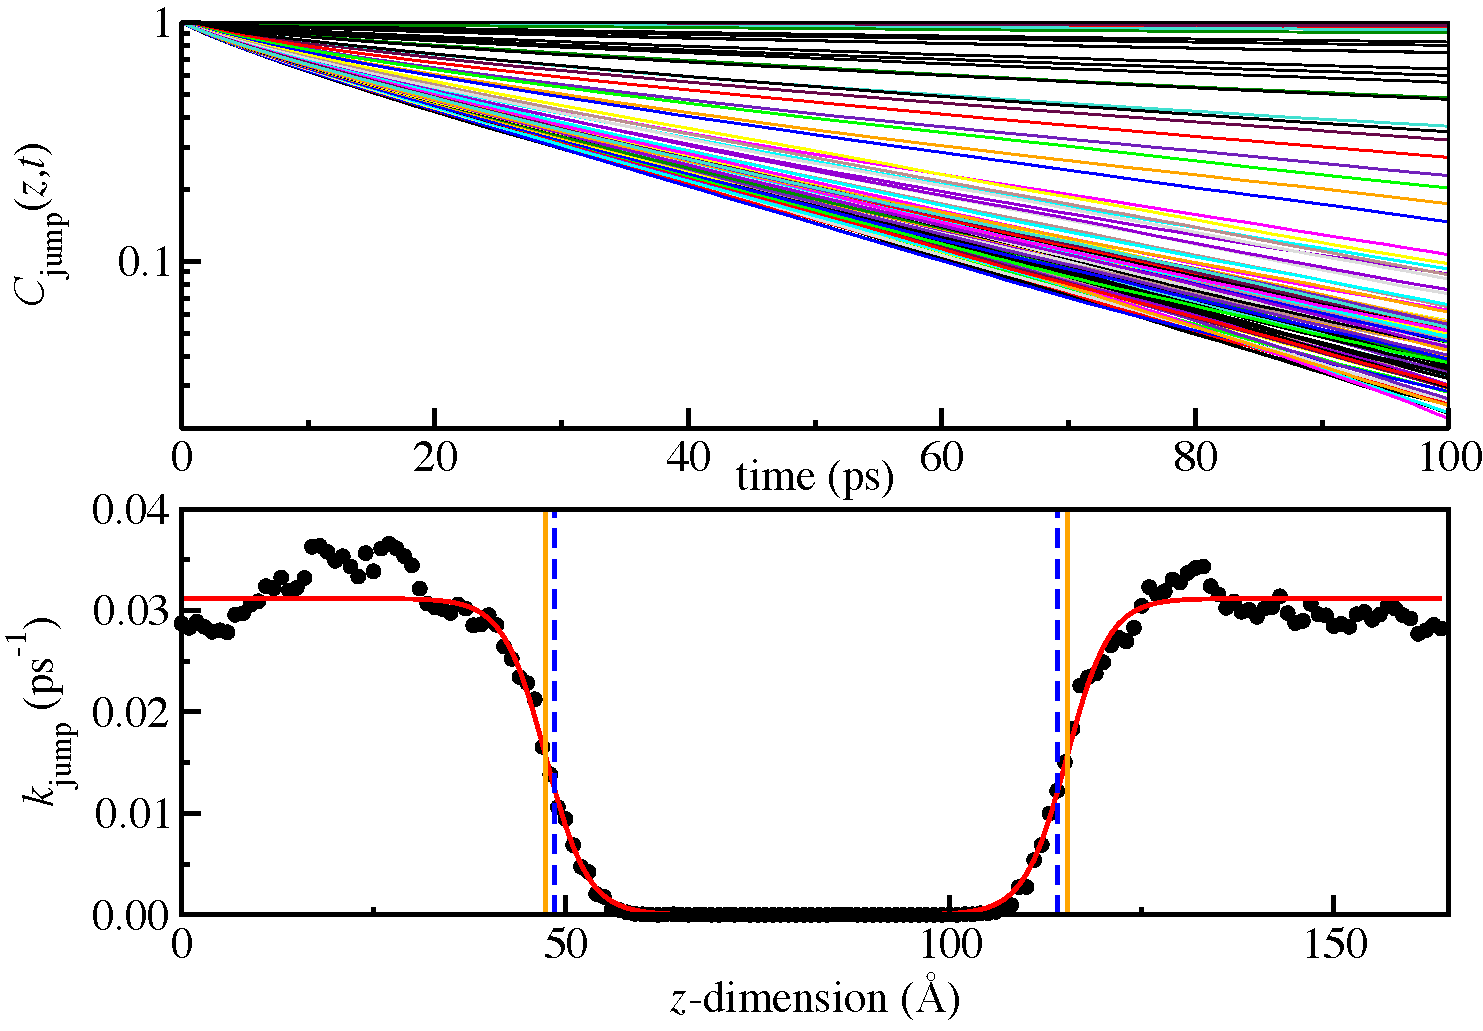
\includegraphics[width=\linewidth]{Figures/secprismJumpPlotTIP4PIce}
\caption{\label{fig:SPTIP4Pkjmp} The same secondary prism hydrogen
  bond jump data as Fig. \ref{fig:SPkjmp}, but collected using the
  TIP4P/Ice model and at 270~K.  Note that the higher coexistence
  temperature for this model increases the observed liquid-state jump
  rates, and has brought the structural and jump interfaces much
  closer together.}
\end{figure}

\subsubsection{A simple model for solid-liquid friction}
The interfacial friction coefficient, $\kappa$ captures the momentum
conductance transverse to the interface, and this momentum should be
transferred via strong intermolecular interactions across the
interface. This is measured in ice / water systems by the surface
density of hydrogen bonds, $\rho_\mathrm{s-l}$.  The momentum is then
carried through the liquid via viscous forces $(\eta)$ across an
interfacial region that has width $w_\mathrm{s-l}$. A simple linear
model,
\begin{equation}
  \kappa = c~~\rho_\mathrm{s-l}~~\eta~~w_\mathrm{s-l},
\label{eq:model}
\end{equation}
captures these features at the ice / water interface, and the results
for the two water models nearly coalesce with a proportionality
constant, $c = 0.343$.  The structural width, $w_\mathrm{10-90}$, and
values for $\eta$ for each ice / water system were obtained by fitting
the liquid portions of the simulation box in conjunction with equation
\eqref{eq:viscosity}.  The two water models have two different
coexistence temperatures, so they exhibit different hydrogen bond
densities and viscosities adjacent to the interface.  Comparing
Eq. \eqref{eq:model} with the non-equilibrium expressions for $\kappa$
(Eq. \eqref{Shenyu-13}) and $\eta$ (Eq. \eqref{eq:viscosity}) shows
that the liquid's viscosity is an important feature in capturing the
velocity drop on the liquid side of the interface
($\eta w_\mathrm{s-l}$), but the magnitude of the solid-liquid
interactions ($c~~\rho_\mathrm{s-l}$) plays a central role in the
observed friction.

\begin{figure}
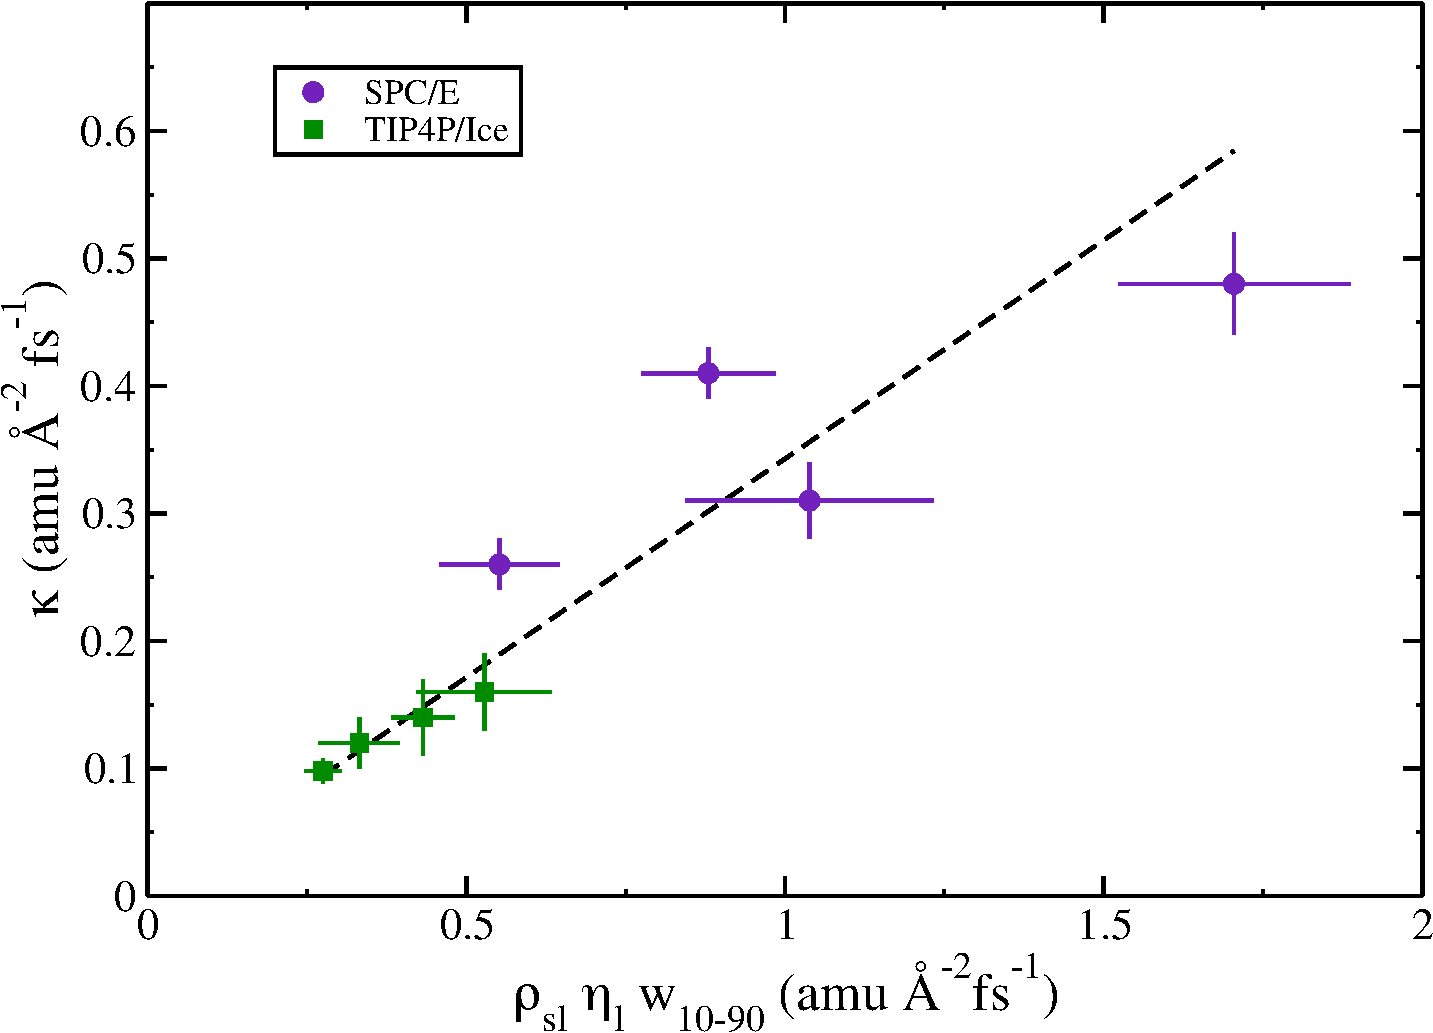
\includegraphics[width=\linewidth]{Figures/simpleModel}
\caption{\label{fig:simpleModel} Solid-liquid friction coefficients
  shown vs. surface hydrogen bond density model (Eq. \eqref{eq:model}
  for all four facets and for both water models.  Although SPC/E
  (225K) and TIP4P/Ice (270K) operate in two distinct viscosity
  domains, the model captures the importance of the density of
  solid-liquid hydrogen bonds.}
\end{figure}                                            

\section{Conclusions}
RNEMD simulations of the different facets of ice being drawn through
surrounding water at the coexistence temperature indicate
facet-dependence of solid / liquid friction.  We have defined a
negative slip interfacial friction coefficient, $\kappa$ (measured in
amu~\AA$^{-2}$ fs$^{-1}$) and find that the two prismatic facets exert
the largest drag on the surrounding liquid.  The basal facet provides
an intermediate level of drag, while the pyramidal facet has roughly
half the interfacial friction of the prismatic facet.

Using the local tetrahedral order parameter as a metric to
differentiate ice and liquid water molecules and a geometric hydrogen
bonding criteria, the friction coefficients were shown to be largely
governed by the surface density of solid / liquid hydrogen bonds
($\rho_{sl}$).  A simple linear model, Eq. \eqref{eq:model}, uses
this density to provide estimates of solid-liquid friction that give
good agrement for two different water models at their respective
coexistence temperatures.

In addition, we have found the ice / water interfacial widths for all
four crystal facets to be similar (using both structural and dynamic
measures) and found these widths to be independent of shear rate.  The
similarity of interfacial width estimates for the four facets indicate
that the particular facet of the exposed ice crystal has very little
effect on how far into the bulk the ice-like structural ordering
persists. While differences have been found in previous simulations of
ice / water interfaces,\cite{Hayward2001,Hayward2002} experimentally
these differences have been less clear.\cite{Beaglehole1993} The
significant differential friction coefficients obtained here suggest
that while the liquid next to the ice might be structurally organized
like bulk liquid, the dynamics of the molecules are still quite
strongly perturbed by the ice.  That is, the surface hydrogen bonding
significantly alters how the water layers are pulled along with the
ice during shear.


